\def\col{blue}
\documentclass[14pt, \col, hyperref={pdfpagelabels=false}]{beamer}
\usepackage[frenchb]{babel} % langue francaise
\usepackage[utf8]{inputenc} % encodage UTF-8
\usepackage[T1]{fontenc} % encodage de la police de caracteres
\usepackage{lmodern}
\usepackage{listings}
\usepackage{multicol}
\usepackage{pifont} %\ding{number}, 
\usepackage{subfigure}
\usepackage{graphicx}
\usepackage{listings}

\usetheme{Warsaw}
\usepackage[\col]{optional} %red blue green
%% THÈMES couleur
%% \usecolortheme{dolphin}
%% \usecolortheme{seahorse}
%% * thèmes globaux : beetle, crane, fly, seagull.
%% * thèmes internes : lily (enlève surtout des couleurs), orchid, rose.
%% * thèmes externes : whale, seahorse, dolphin

% rubber: rules ./rules.ini

 
\mode<presentation>
{
  %%%% Couleurs
  \definecolor{red2}{rgb}{0.8,0.15,0.15}
  \definecolor{bx}{rgb}{0.45,0.05,0.05}  
  \definecolor{ivoire}{rgb}{1, 0.97, 0.9}
 
  \definecolor{bleu2}{rgb}{0.9, 0.90, 1}
  \definecolor{bleu3}{rgb}{0.15,0.15,0.7}
  \definecolor{myblue}{rgb}{0.50,0.55, 0.8}  
  \definecolor{myblue2}{rgb}{0.25,0.3, 0.65}  
  
 \definecolor{mygreen2}{rgb}{0.15,0.60,0.15}
 \definecolor{green2}{rgb}{0.15,0.40,0.15}
  \definecolor{mygreen}{rgb}{0.40,0.7, 0.4}  
%  \definecolor{lightgreen}{rgb}{0.5,0.8, 0.5}  
  \definecolor{lightgreen}{rgb}{0.95, 1, 98}
  
  \definecolor{medium-grey}{gray}{0.45}
  \definecolor{light-grey}{gray}{0.85}
  
  % Couleur des structures et fond dégradé
  % defaut: green
  \setbeamercolor{normal text}{fg=black,bg=lightgreen}
  \setbeamercolor{structure}{fg=green2, bg=light-grey} 
  \setbeamercolor{alerted text}{fg=green2}
  \setbeamertemplate{background canvas}[vertical
    shading][top=lightgreen!100,bottom=lightgreen!30]
  
  \opt{blue}{
    \setbeamercolor{normal text}{fg=black,bg=bleu2}
    \setbeamercolor{structure}{fg=myblue, bg=light-grey} 
    \setbeamercolor{alerted text}{fg=myblue2}
    \setbeamertemplate{background canvas}[vertical
      shading][top=bleu2!100,bottom=bleu2!30]
  }
  \opt{red}{
    \setbeamercolor{normal text}{fg=black,bg=ivoire}
    \setbeamercolor{structure}{fg=bx, bg=light-grey} 
    \setbeamercolor{alerted text}{fg=red2}
    \setbeamertemplate{background canvas}[vertical
      shading][top=ivoire!40,bottom=ivoire!100]
  }
  \opt{green}{
    \definecolor{green2}{rgb}{0.1,0.60,0.1}
    \usecolortheme{dolphin}
  }   
  
  
  \setbeamertemplate{navigation symbols}{}
  \setbeamerfont{title in head/foot}{size=\scriptsize}
  \setbeamerfont{date in head/foot}{size=\scriptsize} 
  
  % Pied de page
  \setbeamertemplate{footline}{
    \hbox{%
      \begin{beamercolorbox}[wd=.4\paperwidth,ht=3ex,dp=1ex,center]{title in head/foot}
        \usebeamerfont{title in head/foot}\enseignement\hspace{1cm} %\shorttitle
      \end{beamercolorbox}%
      \begin{beamercolorbox}[wd=.5\paperwidth,ht=3ex,dp=1ex,left]{date in head/foot}%
        \usebeamerfont{title in head/foot} 
        \hspace*{1ex} 
        \insertshorttitle
      \end{beamercolorbox}% 
      \begin{beamercolorbox}[wd=.1\paperwidth,ht=3ex,dp=1ex,left]{date in head/foot}%
        \usebeamerfont{date in head/foot} 
        \insertframenumber{} / \inserttotalframenumber%\hspace*{2ex} 
    \end{beamercolorbox}}%
    \vskip0pt%
  }

    % Haut de page
  \setbeamertemplate{headline}{%
    \leavevmode
    \begin{beamercolorbox}[wd=.5\paperwidth,ht=3ex,dp=1.125ex,leftskip=.3cm
        plus1fill,rightskip=.3cm]{section in head/foot}%
      \scriptsize{\insertsection}
    \end{beamercolorbox}%
    \begin{beamercolorbox}[wd=.5\paperwidth,ht=3ex,dp=1.125ex,leftskip=.3cm,rightskip=.3cm
        plus1fil]{subsection in head/foot}%
      \scriptsize{\insertsubsection}
    \end{beamercolorbox}%
  }
  \addtobeamertemplate{headline}{}{%
    \vskip-0.1pt
    \pgfuseshading{beamer@topshade}
    \vskip-2pt}
   %% \let\Tiny=\tiny
  %% \let\TINY=\tiny
}

%% Annonce de plan a chaque transition.
%% \AtBeginSection[]{
%%   \begin{frame}<beamer>
%%     \frametitle{Plan}
%%     \tableofcontents[currentsection,currentsubsection]
%%   \end{frame}
%% }



\newcommand{\bashlisting}[0]{\scriptsize\lstset{language=bash,numbers=left,numberstyle=\tiny,
    xrightmargin=1mm, xleftmargin=1mm, keywordstyle=\color{green2}, %
    keywordstyle[1]=\color{blue}, %
    keywordstyle[2]=\color{yellow}, %
    keywordstyle[3]=\color{red2}}}

\newcommand{\filelisting}[0]{\small\lstset{language=,numbers=left,numberstyle=\tiny,
    xrightmargin=4mm, xleftmargin=6mm, frame=single}}

\definecolor{orange}{rgb}{0.9,0.6,0.4}

\newcommand{\clisting}[0]{\scriptsize
  \lstset{language=c, 
    inputencoding=utf8,
    %identifierstyle=\color{blue},%
    keywordstyle=\color{green2}, %
    keywordstyle[1]=\color{blue}, %
    keywordstyle[2]=\color{yellow}, %
    keywordstyle[3]=\color{red2}, %
    stringstyle=\color{orange}, %
    commentstyle=\color{red2}, %
    numbers=left,
    numberstyle=\tiny,
    xleftmargin=1mm,
    breaklines=true,
}}



\newcommand{\cmd}[1]{\texttt{\footnotesize\textcolor{medium-grey}{#1}}}

\newcommand{\cmdlist}[1]{
  \begin{semiverbatim}\begin{minipage}{\linewidth}  
      \footnotesize\textcolor{medium-grey}{#1}\end{minipage}
\end{semiverbatim}}


\newcommand{\coeur}{c\oe ur\xspace}
\newcommand{\oeuvre}{\oe uvre\xspace}
\newcommand{\coeurs}{c\oe urs\xspace}
\newcommand{\mc}{multic\oe ur\xspace}
\newcommand{\mcs}{multic\oe urs\xspace}

\usepackage{multicol}

%%%%%%%%%%%%%
\def\enseignement{ASR2 Système}
\title[]{%\enseignement\\
Gestion de la mémoire}
\author{Stéphanie Moreaud}
\institute{Département d'informatique\\
  IUT Bordeaux 1}
\date{}

%%%%%%%%%%%% 
   
\newcommand{\TITRE}[1]{
  \begin{frame}
    \begin{center}\huge{#1}\end{center}
\end{frame}
}


\newcommand{\FIGURE}[2]{
  \begin{frame}
    \frametitle{\insertsubsection}
    \begin{figure}
    \includegraphics[width=0.8\linewidth]{memoire-images/#1}
    \end{figure}
    \begin{center}\large{#2}\end{center}
    
  \end{frame}
}
%%%%%%%%%%%%%%%%%%%%%%%%%%%%%%%%%%%%%ù
\begin{document}

\begin{frame}
  \titlepage
\end{frame}

%%%%%%%%%%%%%%%%%%%%%%%
\begin{frame}<beamer>
  \frametitle{Plan}
  \begin{columns}[t]
    \begin{column}{5cm}
      \tableofcontents[sections={1-5},currentsection, hideothersubsections]
    \end{column}
    \begin{column}{5cm}
      \tableofcontents[sections={6-10},currentsection,hideothersubsections]
    \end{column}
  \end{columns}
  
 % \tableofcontents[hideallsubsections]
\end{frame}
%%%%%%%%%%%%%%%%%%%%%%%%%

%Annonce de plan a chaque transition.
\AtBeginSection[]{
  \begin{frame}<beamer>
    \frametitle{Plan}
    \begin{columns}[t]
      \begin{column}{5cm}
        \tableofcontents[sections={1-5}, currentsection, hideothersubsections]
      \end{column}
      \begin{column}{5cm}
        \tableofcontents[sections={6-10},currentsection,hideothersubsections]
      \end{column}
    \end{columns}
  \end{frame}
}

\begin{frame}
\frametitle{Bibliographie}
\bibliographystyle{fr-plain}
\small
\nocite{*}    
\bibliography{bib}  
\vspace{0.5cm}    
Remerciements à Michel Billaud.
\end{frame}


\section{Introduction}
\begin{frame}
\frametitle{Ressource mémoire}
\alert{Mémoire}~: ressource essentielle au fonctionnement d'un ordinateur qui permet
    le stockage des informations. \\
\vspace{0.5cm}

L'évolution des ordinateurs s'accompagne de l'augmentation de la puissance de calcul
et de la mémoire disponible... \\
... mais plus il y a de ressources disponibles, plus les programmes sont gourmands. \\
%\vspace{0.5cm}
\begin{itemize}
\item les besoins en mémoire augmentent aussi vite que la taille de celle-ci...
\item[\ding{212}] la mémoire doit être gérée avec soin. \\
\end{itemize}

\vspace{0.5cm}
\alert{Objectif du cours}~: comprendre comment les systèmes d'exploitation gèrent la mémoire.  
\end{frame}


\begin{frame}
\frametitle{Ressource mémoire}
Les programmeurs voudraient une mémoire~:
\begin{itemize}
\item infiniment grande
\item extrêmement rapide
\item non volatile  
\item bon marché
\end{itemize}
\ding{212} de telles mémoires n'existent pas...\\
\vspace{0.5cm}

On utilise des compromis 
\begin{itemize}
\item plusieurs types de mémoire, différentes caractéristiques
\begin{itemize}
\item très rapide / moins rapide
\item volatile / non volatile
\item chère / bon marché
\end{itemize}
\item organisation hiérarchique
\end{itemize}
\end{frame}


\begin{frame}
  \frametitle{Hiérarchie mémoire}
  L'information est stockée dans plusieurs niveaux de mémoire
  \begin{itemize}
  \item \alert{Registres}
    \begin{itemize}
    \item interne au CPU, capacité < 1Ko, gérés par le programme
    \end{itemize}
  \item \alert{Mémoire cache}
    \begin{itemize}
    \item très rapide, très chère, capacité de quelques Mo. 
    \end{itemize}
  \item \alert{Mémoire principale} (\emph{Random Access Memory})
    \begin{itemize}
    \item assez rapide, chère, capacité allant jusqu'à quelques dizaines de
      Go pour les gros calculateurs  
    \end{itemize}
  \item \alert{Disque dur}
    \begin{itemize}
    \item lent, peu chère, grande capacité (centaines de Go), non volatile 
    \end{itemize}
  \item \alert{Bande magnétique}
    \begin{itemize}
    \item très grande capacité, très peu chère, accès très
      lent, durée de vie longue. 
    \item utilisé pour l'archivage, concurrencé par les disques 
    \end{itemize}
  \end{itemize}
\end{frame}

\subsection{Systèmes et mémoire}
\begin{frame}
  \frametitle{Systèmes monotâches}
  \alert{Système monotâche} \ding{212} 1 seul programme en mémoire\\
  \vspace{0.5cm}
  Utilisation de cartes perforées
  \begin{itemize}
  \item lecteur de carte remplissait la mémoire
  \item machine dans une salle entière
  \item fastidieux
  \end{itemize}
  Apparition des bandes magnétiques
  \begin{itemize}
  \item programme chargé en mémoire exécute les calculs et fait des opérations d'E/S
  \item[\ding{212}] chargement de données à l'exécution
  \item lecture sur la bande magnétique très lente
  \end{itemize}
\end{frame}

\begin{frame}
  \frametitle{Systèmes multitâches}
  \alert{Système multitâche} \ding{212} plusieurs programmes chargés en mémoire\\
  \vspace{0.5cm}
  
  La \alert{cohabitation} dans l'\alert{espace mémoire}
  introduit de nouvelles problématiques
  \begin{itemize}
  \item Comment partager la mémoire entre les différents programmes? Éviter le
    gaspillage? 
  \item Comment protéger les programmes les uns des autres? 
  \item Comment assurer le fonctionnement des programmes sans compliquer la
    programmation? 
  \end{itemize}
\end{frame}



\section{Partage de la mémoire}
\begin{frame}
\frametitle{\insertsection}
Où mettre les programmes?\\
\vspace{0.5cm}
Idée~: partitionner la mémoire
\begin{itemize}
\item mémoire physique divisée statiquement en partitions fixes
\item programme chargé dans dans une zone suffisamment grande 
\item facile à implémenter, peu coûteux. 
\item gaspillage de mémoire, nombre de programmes limités
\end{itemize}
\vspace{0.5cm}
\pause Autre idée~: les uns à la suite des autres
\begin{itemize}
\item[\ding{212}] allocation contiguë
\item partition de taille dynamique
\item création à la volée en fonction de la mémoire requise, taille optimale
\end{itemize}
\end{frame}

\subsection{Allocation contiguë}
\begin{frame}
  \frametitle{Allocation contiguë}
Pour chaque processus, un espace \alert{contigu} en mémoire physique
\begin{itemize}
\item[\ding{212}] une plage d'adresses
\end{itemize}
\vspace{0.5cm}
\begin{figure}
  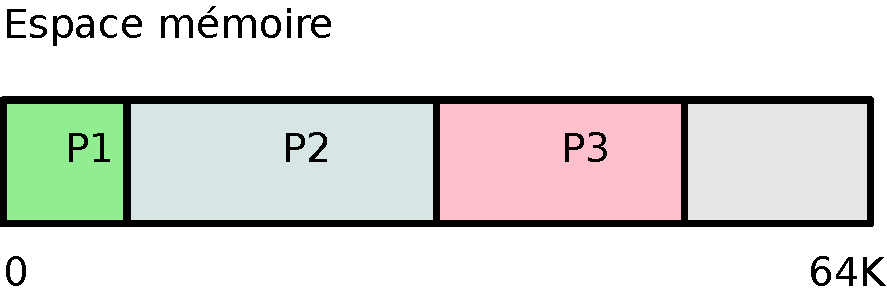
\includegraphics[width=0.8\linewidth]{fig2/dia-partage-memoire}
\end{figure}
\end{frame}

\begin{frame}
  \frametitle{L'allocation contiguë}
  Problèmes~:
  \begin{itemize}
  \item Emplacement du code connu au \alert{chargement}
  \item[\ding{212}] Le code doit être \alert{indépendant} de sa position physique.
  \vspace{0.5cm}
  \item Les espaces \alert{alloués} sont 
    \begin{itemize}
    \item de \alert{tailles diverses}
    \item \alert{libérés} dans un ordre imprévisible 
    \end{itemize}
  \item[\ding{212}] Comment gérer les allocations/restitutions des espaces~?    
  \end{itemize}
\end{frame}


\section{Adresses logiques}

%% \begin{frame}
%% \frametitle{Indépendance code/position}

%% \item Problème : Indépendance code / position
%% \item solution : adresses logiques
%% \item mécanisme de génération d'adresses
%% \item protection de la mémoire
%% \end{frame}

\subsection{Indépendance code/position physique}


\begin{frame}
  \frametitle{Indépendance code /position}
  Pb~: Un exécutable peut être \alert{chargé} à des emplacements
  différents (éventuellement simultanément)
  \vspace{0.5cm}
  \begin{figure}
    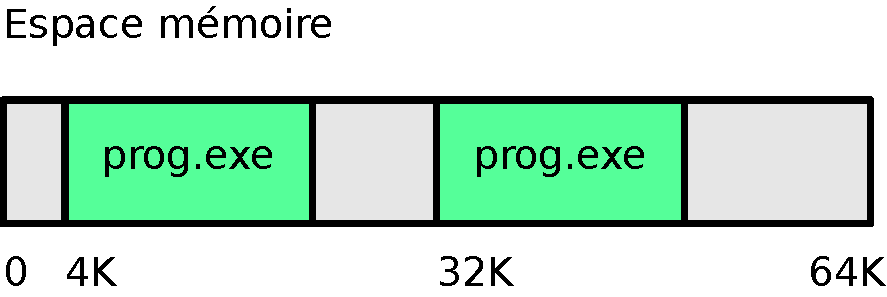
\includegraphics[width=0.8\linewidth]{fig2/indep-code-adr-physique}
  \end{figure}
  \vspace{0.5cm}
  Il doit fonctionner sans modification.
\end{frame}

\begin{frame}
  \frametitle{\insertsubsection}
  Chaque processus utilise des \alert{adresses logiques}. \\
  
  Le compilateur génère du \alert{code relatif} au début du programme
  \begin{itemize}
  \item toutes les adresses sont exprimées comme si le programme était chargé à
    l'adresse 0
  \item[\ding{212}] l'\alert{espace mémoire logique} d'un processus commence à
    \underline{son} adresse zéro 
  \end{itemize}
\end{frame}

\begin{frame}
  \frametitle{\insertsubsection}
  \begin{figure}
    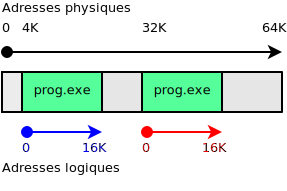
\includegraphics[width=0.7\linewidth]{fig2/indep-code-adr-logique}
  \end{figure}
  Il faut alors traduire l'\alert{adresse logique} utilisée dans le code en
  l'\alert{adresse physique} correspondante dans la mémoire. \\
  \vspace{-0.5cm}
$$adresse~physique = adresse~de~base~ +~ adresse~logique$$
\end{frame}

\subsection{Conversion adresse logique/adresse Physique}

\begin{frame}
  \frametitle{Conversion adresse logique/adresse physique}
  
  \underline{Première solution~}: conversion au chargement
\begin{itemize}
\item Le compilateur maintient une liste de tous les endroits du
  où l'on effectue une manipulation d'adresse. 
\item Au chargement, le système doit corriger les adresses en fonction de
  l'adresse de chargement du programme en suivant les indications du compilateur.   
\end{itemize}
\begin{itemize}
\item[\ding{212}] faisable mais coûteux
\item[\ding{212}] aucune protection mémoire 
\end{itemize}
 
\end{frame}

\begin{frame}
  \frametitle{Conversion adresse logique/adresse physique}
  \frametitle{Modification du matériel}
  \underline{Deuxième solution}~: conversion à l'exécution
  \begin{itemize}
  \item[\ding{212}] \alert{Alternative matérielle}
  \item le \alert{registre de base} contient l'adresse de chargement du programme en
    mémoire.
  \item un \alert{additionneur} ajoute à l'adresse logique la valeur du registre de
    base.  
  \end{itemize}
  \begin{figure}
    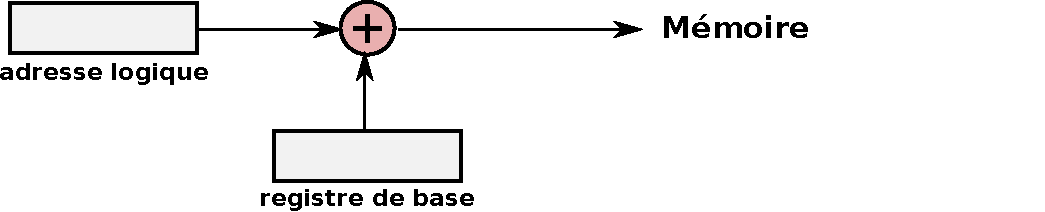
\includegraphics[width=\textwidth]{fig2/conv-log-phys}
  \end{figure}
\end{frame}

\subsection{Protection inter-processus}

\begin{frame}
\frametitle{\insertsubsection}
Comment éviter qu'un processus n'accède à l'espace mémoire d'un autre? \\
\vspace{0.5cm}
\pause
Une adresse logique \alert{valide} est comprise entre
\begin{itemize}
\item 0
\item la taille de l'espace logique (-1)
\end{itemize}
\ding{212} comparer l'adresse logique avec la taille de l'espace logique. 
\end{frame}

\begin{frame}
  \frametitle{\insertsubsection}
  Modification du matériel~: vérification des adresses logiques
  \begin{itemize}
  \item le \alert{registre de limite} contient la taille
    de l'espace logique du processus en cours
  \item un \alert{comparateur} effectue la comparaison  entre l'adresse logique et la
    valeur du registre de limite
  \item[\ding{212}] génère une interruption si dépassement
  \end{itemize}
  \begin{figure}
    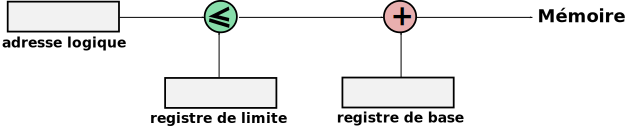
\includegraphics[width=\linewidth]{fig2/conv-log-phys2}
  \end{figure}    

\end{frame}

\subsection{Bilan}
\begin{frame}
\frametitle{Adresses logiques~: Bilan}
Introduction des \alert{adresses logiques} 
\begin{itemize}
\item code indépendant de sa position en mémoire
\item simplifie le chargement des programmes 
\item facilite leur protection 
\end{itemize}

Nécessite la conversion en adresse physique (réelle) 
\begin{itemize}
\item réalisée par le \alert{matériel}
\item simple (utilisation de registres, additionneur, comparateur)
\item à faible coût
\end{itemize}
\end{frame}

% ------------------------------------------------------------
\section{Gestion de l'allocation contiguë}
\subsection{Fragmentation}
\begin{frame}
  \frametitle{Gestion de l'allocation contiguë}
  Initialement~: un espace physique \alert{libre} en mémoire\\
  \vspace{0.5cm}
  Évolution du traitement des programmes 
  \begin{itemize}
  \item \alert{allocations} de zones (prises dans l'espace libre)
  \item \alert{libération} de zones allouées 
  \end{itemize}
\vspace{0.5cm}
\ding{212} problème de \alert{fragmentation}
\begin{itemize}
\item allocations/libérations faites dans un ordre imprévisible
\item tendance à laisser des \alert{trous}
\item les trous trop petits sont inexploitables
\end{itemize}
\end{frame}


%% \subsection{Exemple de scénario}
\begin{frame}
\frametitle{\insertsubsection}
\begin{figure}[h]
  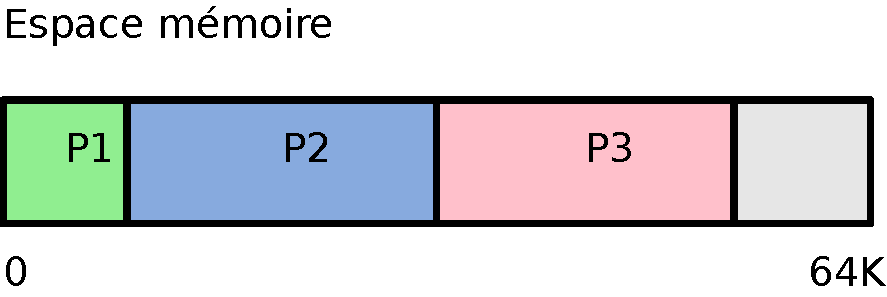
\includegraphics[width=0.8\textwidth]{fig2/frag-1}
\end{figure}
\center{\large(0) 3 processus sont présents, P2 se termine ...}
\end{frame}


\begin{frame}
\frametitle{\insertsubsection}
\begin{figure}[h]
  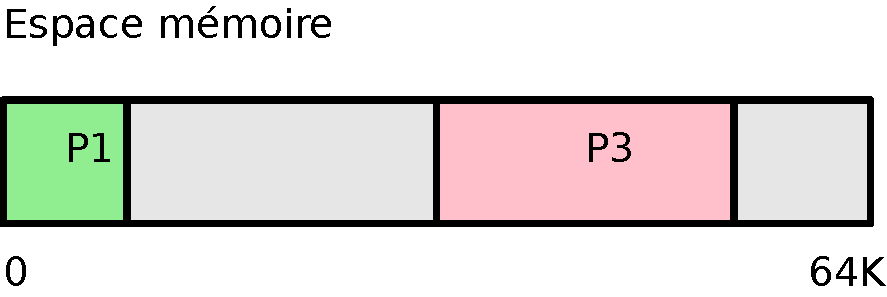
\includegraphics[width=0.8\textwidth]{fig2/frag-2}
\end{figure}
\center{\large (1) allocation de P4 ...}
\end{frame}

\begin{frame}
\frametitle{\insertsubsection}
\begin{figure}[h]
  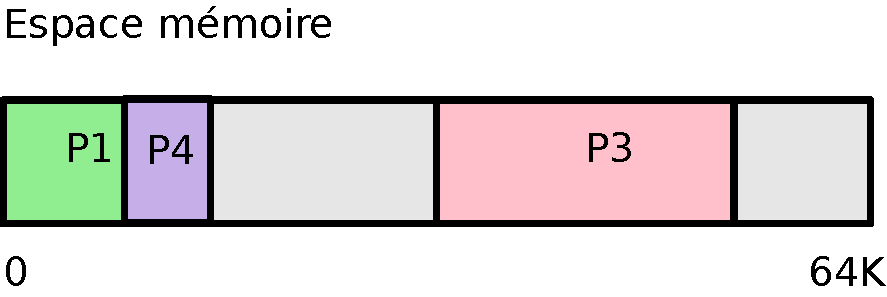
\includegraphics[width=0.8\textwidth]{fig2/frag-3}
\end{figure}
\center{\large (3) allocation de P5 ...}
\end{frame}

\begin{frame}
\frametitle{\insertsubsection}
\begin{figure}[h]
  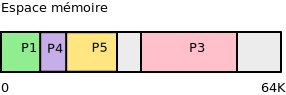
\includegraphics[width=0.8\textwidth]{fig2/frag-4}
\end{figure}
\center{\large (4) libération de P4 ...}
\end{frame}

\begin{frame}
\frametitle{\insertsubsection}
\begin{figure}[h]
  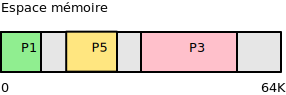
\includegraphics[width=0.8\textwidth]{fig2/frag-5}
\end{figure}
\center{\large(5) l'espace libre est fragmenté}
\end{frame}

 \subsection{Solutions}
\begin{frame}
  \frametitle{Remèdes à la fragmentation}
  \underline{Solution curative~:} \alert{compactage} (relocation)
  \begin{itemize}
  \item \alert{translater} les zones allouées pour reconstituer une grande zone libre   
  \item nécessite de lire toute la mémoire \ding{212} terriblement coûteux 
  \end{itemize}
  
  \vspace{0.5cm}
  \underline{Technique préventive~:} choix de la stratégie d'allocation
    \begin{itemize}
    \item first-fit, best-fit, worst-fit ...
    \end{itemize}
\end{frame}

\begin{frame}
  \frametitle{\insertsubsection}
  \begin{itemize}
  \item \alert{first-fit}~: allocation dans le premier bloc assez grand pour contenir
    le programme
    \begin{itemize}
    \item le reste devient une zone libre plus petite
    \end{itemize}
  \item \alert{best-fit}~: allocation dans le plus petit bloc qui soit assez grand
    \begin{itemize}
    \item méthode est plus coûteuse, évite de couper inutilement une grande zone,
      génère plus vite de très petites zones
    \end{itemize}
  \item \alert{worst-fit} allocation dans le plus grand bloc
    \begin{itemize}
    \item limite les trop petites zones, pénalisant pour les gros programmes
    \end{itemize}
  \item autres stratégies (buddy system, quick-fit)
  \end{itemize}
\end{frame}

\subsection{Bilan}
\begin{frame}
\frametitle{\insertsubsection}

L'allocation de zones \alert{contiguës} de tailles diverses conduit à la
\alert{fragmentation}

\begin{itemize}
\item problème retrouvé ailleurs (gestion des disques,
 \texttt{new}, \texttt{delete} en programmation, ...)
\item les solutions préventives et curatives
  sont plus ou moins satisfaisantes
\end{itemize}
\end{frame}


% -----------------------------------------------
\section{Swapping}
\begin{frame}
  \frametitle{Swapping (va-et-vient)}
  La mémoire principale est une ressource limitée\\
  \ding{212} peut être insuffisante pour maintenir tous les processus courants 
  (système à temps partagé)\\
 
  \vspace{0.5cm}
  Idée~: conserver les processus supplémentaires sur le disque et les recharger pour
  les exécuter.
  \begin{itemize}
  \item transférer sur disque les processus inactifs
  \item les ramener le moment voulu
  \end{itemize}
 \end{frame}

\begin{frame}
\frametitle{Swapping}
\begin{figure}[h]
  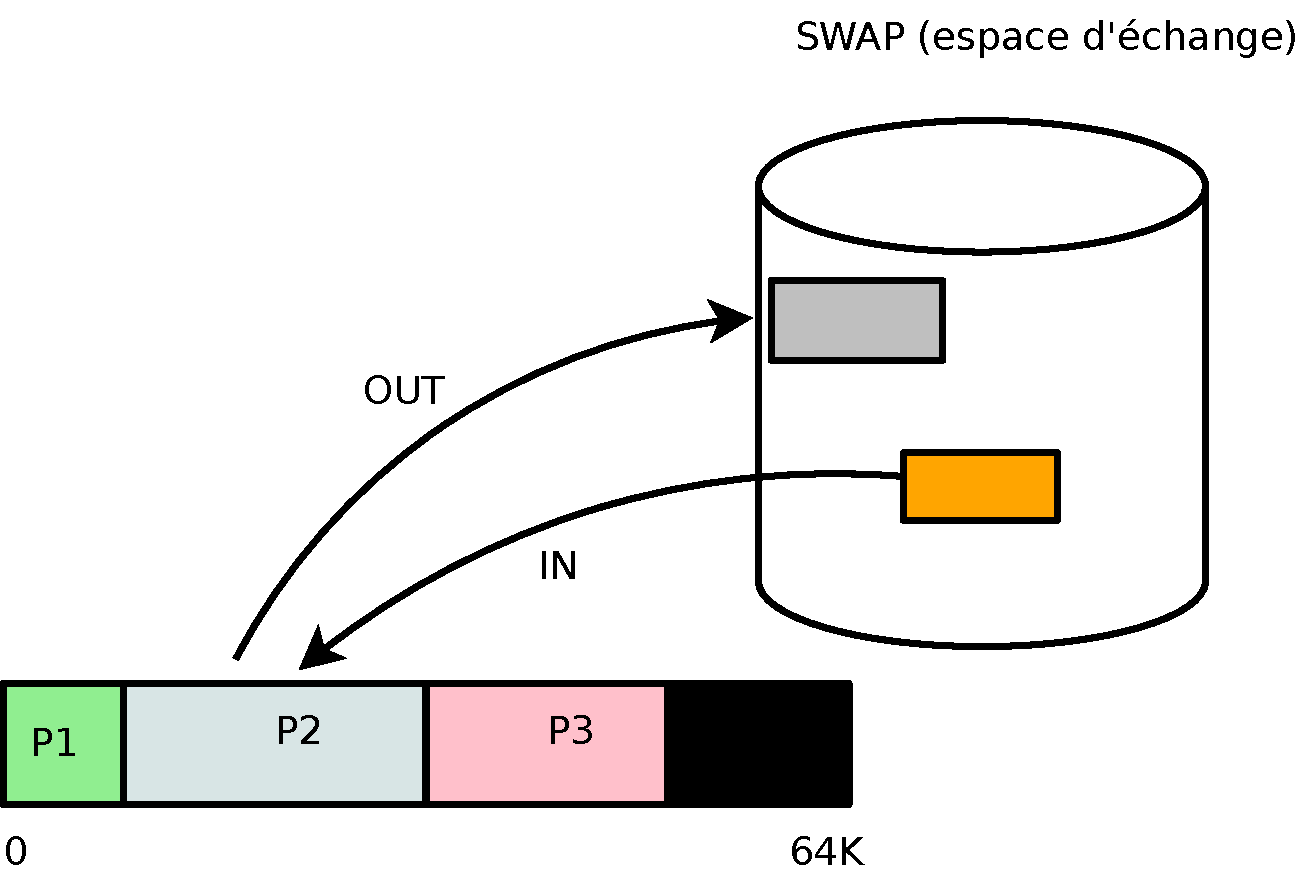
\includegraphics[width=0.8\textwidth]{fig2/swapping-segment}
\end{figure}
\center{Échanges mémoire \ding{214} disque}
\end{frame}

\begin{frame}
\frametitle{Avantages}
On peut charger plus de processus en \alert{mémoire virtuelle} que la mémoire
centrale ne peut en contenir\\ 
\vspace{0.5cm}
Permet d'attendre des taux de charge élevés (rentabilisation)\\
\vspace{0.5cm}
Viable pour les applications interactives,
l'utilisateur est un périphérique très lent\\
\end{frame}

% -------------------------------------------------

\section{Segmentation}
\subsection*{Segmentation}

\begin{frame}
  \frametitle{Segmentation}
\underline{Principe}~: diviser l'espace mémoire en espaces logiquement indépendants (segments)\\  
\vspace{0.3cm}
L'espace mémoire d'un processus comporte au moins deux \alert{segments} :
\begin{itemize}
\item le segment de \alert{code}
\begin{itemize}
\item commun aux différentes instances du programme 
\item un seul instance du code en mémoire, segment \alert{partagé} entre les processus
\end{itemize}
\item le segment de \alert{données}
  \begin{itemize}
  \item différent pour chaque processus
  \end{itemize}
\end{itemize}
\vspace{0.3cm}
\underline{Avantages~}: partage segment (code, bibliothèque), économie mémoire, droits d'accès différents, ...\\
\end{frame}

\begin{frame}
\frametitle{\insertsubsection}
\begin{figure}
  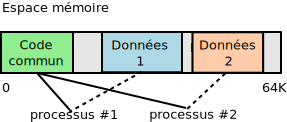
\includegraphics[width=0.8\linewidth]{fig2/seg1}
\end{figure}
Deux processus exécutent le même code
\end{frame}

\begin{frame}
\frametitle{\insertsubsection}
Plusieurs \alert{segments} \ding{212} position différentes en mémoire.\\
\vspace{0.5cm}
\underline{Adresse logique} contient le couple:
\alert{$$<num\_segment, offset>$$}\\
\vspace{-0.4cm}
\begin{itemize}
\item \emph{num\_segment} = \alert{numéro de segment}
\item \emph{offset} = position (déplacement) dans le segment
\end{itemize}
\vspace{0.3cm}
La \alert{table des segments} permet d'effectuer la translation entre adresse logique
et adresse physique\\
\vspace{0.3cm}

Chaque entrée de la table contient~:
\begin{itemize}
\item l'\alert{adresse de base} du segment,
\item la \alert{taille} (longueur) du segment.
\end{itemize}

%%  Segment-table base register (STBR) pointe sur la table des
%% ségments en mémoire\\
%%  Segment-table length register (STLR) indique le nombre de
%% ségments utilisés par un processus;
\end{frame}

\begin{frame}
  \frametitle{Tables des segments}
\begin{figure}[h]
  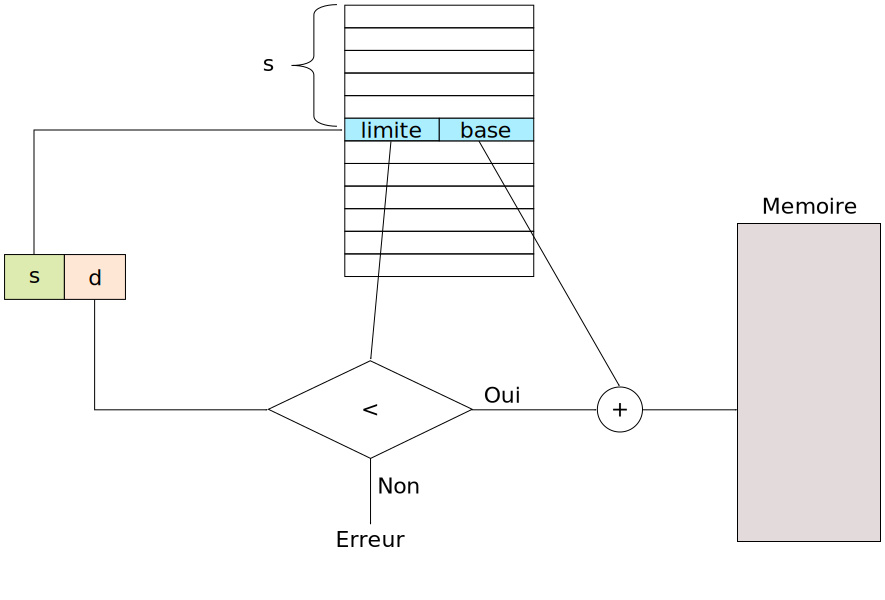
\includegraphics[width=\textwidth]{fig2/segmentation}
\end{figure}
\vspace{-0.5cm}
\small{source~: \href{http://fr.wikipedia.org/wiki/Fichier:Vm7.svg}{\textcolor{blue}{Wikipedia}}}
\end{frame}

%% Utilité de la segmentation

%% La segmentation permet la séparation des données et du programme (entre autres
%% segments) dans des espaces logiquement indépendants facilitant alors la
%% programmation, l'édition de liens et le partage interprocessus. La segmentation
%% permet également d'offrir une plus grande protection grâce au niveau de privilège
%% de chaque segment (voir Descripteur de segment). 

\begin{frame}
\frametitle{Remarque~: numéros de segments}

On distingue la numérotation de segment
\begin{itemize} 
\item locale~: propre à chaque processus
\item globale~: commune
\end{itemize}

Deux processus peuvent utiliser le même segment réel 
avec des numéros locaux (éventuellement) différents.

Remarque~:\\
\begin{itemize}
\item La \alert{table locale des segments} (TLS) d'un processus
fournit le \alert{numéro de segment global} à partir du
\alert{numéro de segment local}
\item La \alert{table globale de segments} (TGS) contient la description de
chaque segment (longueur, pages, protections ...)
\end{itemize}
\end{frame}

\subsection{Bilan}
\begin{frame}
  \frametitle{Bilan}
  
  La segmentation permet le découpage mémoire d'un programme en plusieurs segments logiques.
  \begin{itemize}
  \item \alert{adresse logique} représentée par un numéro de segment et une position
  \item utilisation d'une \alert{table des segments}
  \item permet un gain de place important~: 
    \begin{itemize}
    \item évite la duplication de code, segments utilisés pour les \alert{bibliothèques communes}.
    \end{itemize}
  \end{itemize}
\end{frame}



% ---------------------------

\section{Espace mémoire paginé}
\begin{frame}
  \frametitle{Espace mémoire paginé}
 
  \underline{Contexte}~: Partage de la mémoire physique par des processus
  \underline{Problème}~: fragmentation causée par l'allocation et la libération
  d'espaces de tailles diverses \ding{212} gaspillage de mémoire.  
  
  \underline{Idée}~: déporter le problème à l'intérieur des processus
  \begin{itemize}
  \item espace découpé en \alert{pages de mêmes tailles}
  \item les pages d'un même espace ne sont pas forcément consécutives
  \item la \alert{table des pages} indique la position en mémoire 
    des pages d'un processus
  \end{itemize}
  \ding{212} \alert{Pagination}
\end{frame}

\begin{frame}
\frametitle{Pagination}
Espaces logiques découpés en \alert{pages logiques}~: souvent 4Ko.\\
\vspace{0.3cm}
La mémoire physique est découpée en \alert{cadres de pages} de la même taille.\\
\vspace{0.3cm}
Adresse logique comprend~: le numéro de page et la position dans la page. 
\begin{figure}
  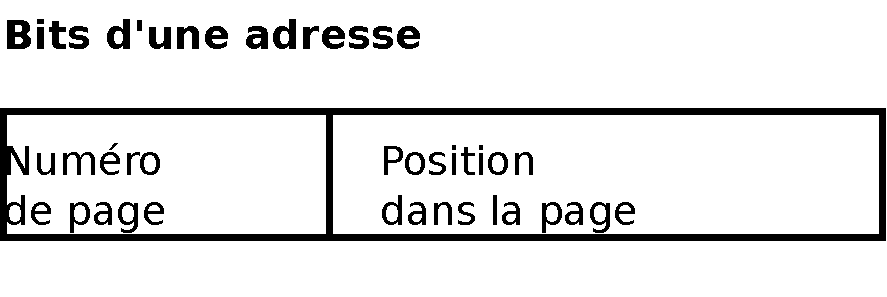
\includegraphics[width=0.5\linewidth]{fig2/format-pagination}
\end{figure}
Pour chaque processus, la \alert{table des pages} permet de retrouver la
correspondance avec l'adresse physique.
\end{frame}

\begin{frame}
\frametitle{Espace paginé}
\begin{figure}
  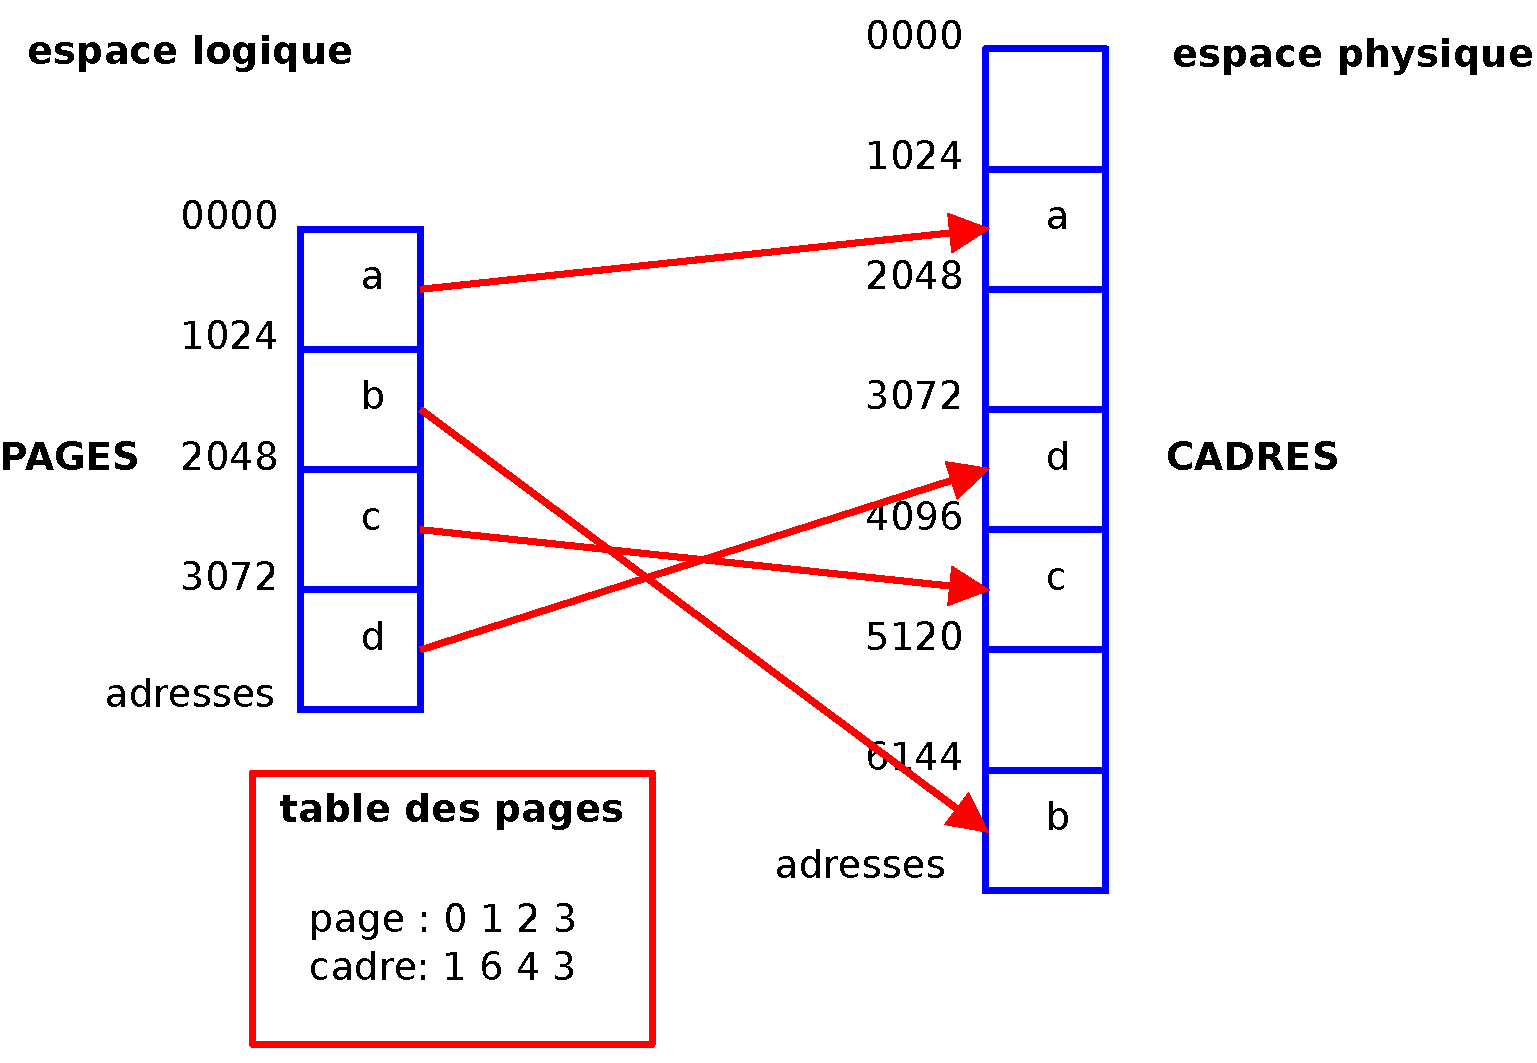
\includegraphics[width=\linewidth]{fig2/pagination}
\end{figure}
\end{frame}

\begin{frame}
  \frametitle{Génération d'adresses}
  Le \alert{numéro de page} est codé par les bits de poids forts
  \begin{itemize}
  \item il est converti en numéro de \alert{cadre de page}
  \end{itemize}
  Les bits de poids faible donnent la \alert{position dans la page}
  \begin{itemize}
  \item cadre de page et page logique de même taille\\
    \ding{212} déplacement équivalent 
  \end{itemize}
  \begin{figure}
    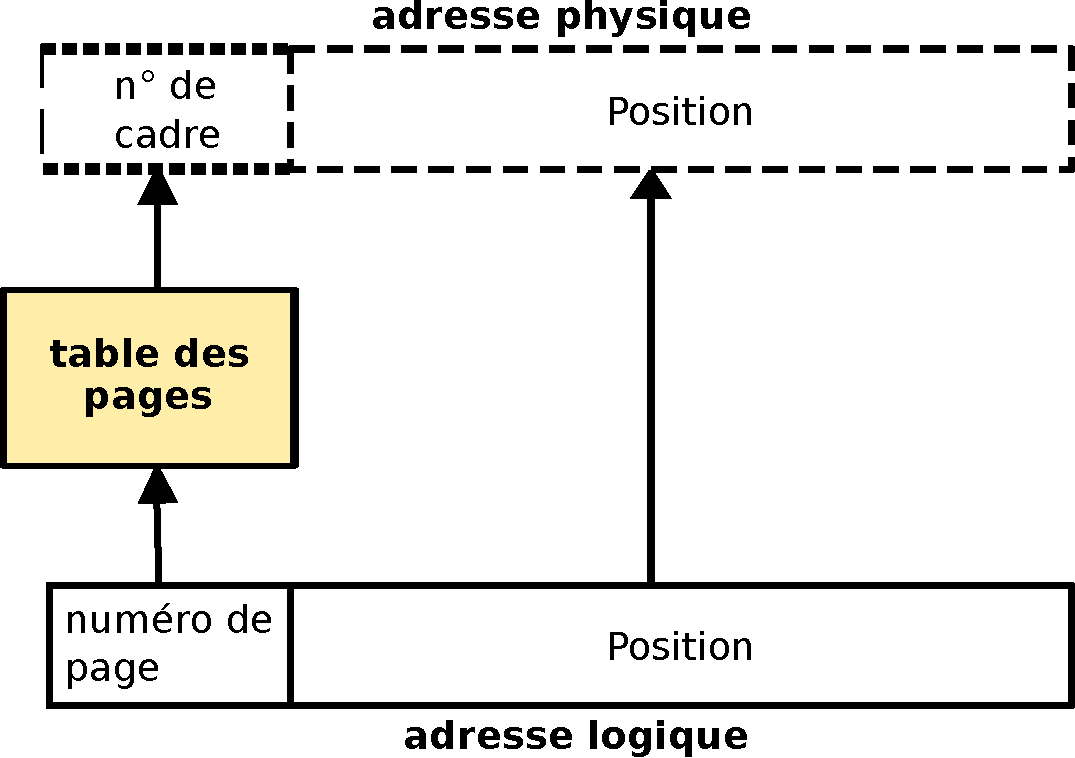
\includegraphics[width=0.6\linewidth]{fig2/generation-pagination}
  \end{figure}
\end{frame}


\section{Mémoire virtuelle paginée}
\begin{frame}
  \frametitle{Mémoire virtuelle paginée}
  \underline{Principe}~: combinaison de la pagination et du swapping.  
  \begin{itemize}
  \item la table des pages connaît les pages présentes 
  \item interruption en cas de \alert{défaut de page} (la page référencée n'est pas en mémoire)
  \end{itemize}
\end{frame}

\subsection{Unité de Gestion Mémoire (MMU)}
\begin{frame}
  \frametitle{\insertsubsection}

  Circuit spécialisé \alert{Memory Management Unit}\\
 
  En charge de~:
  \begin{itemize}
  \item la translation d'adresses logiques (virtuelles) en adresses physique
  \item La protection mémoire 
  \item contrôle de cache
  \item l'arbitrage du bus
  \end{itemize}
\end{frame}


\begin{frame}
  \frametitle{En cas de défaut de page}
  Le système d'exploitation reprend la main 
  \begin{itemize}
  \item S'il y a des cadres vides, il ramène les pages demandées. 
  \item Sinon il évacue une page sur disque pour libérer un emplacement
    \vspace{0.5cm}
  \item il installe la page manquante, 
  \item met à jour la MMU
  \item et relance l'instruction interrompue.
  \end{itemize}
\end{frame}


\begin{frame}
  \frametitle{Swapping}
  \begin{figure}
    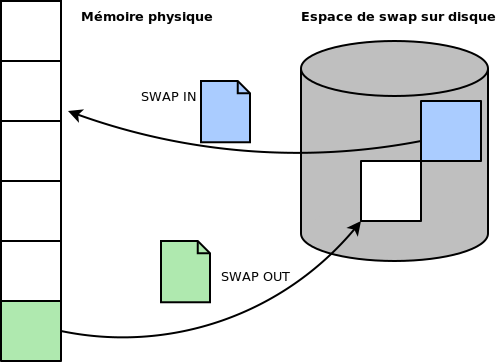
\includegraphics[width=0.8\linewidth]{fig2/swapping}
  \end{figure}
\end{frame}

\section{Algorithmes de remplacement de page}
\begin{frame}
  \frametitle{Algorithmes de remplacement de page}
  \textbf{Comment choisir la page à remplacer ?}
  Idéal~: choisir la page qui sera utilisée le plus tard possible (voir
  plus du tout).\\
  
  Pour choisir un emplacement à libérer, en général on choisit les pages
  \emph{les moins utiles}\\
  \vspace{0.5cm}
  Plusieurs algorithmes~:
  \begin{itemize}
  \item FIFO
    %% \begin{itemize}
    %% \item liste des pages présentes ordonnée par date d'apparition
    %% \item la plus ancienne est choisie
    %% \end{itemize}
  \item LRU (Least Recently Used) 
    %% \begin{itemize}
    %% \item on choisit une page inutilisée depuis lontemps
    %% \item date d'apparition concervée, implémentation coûteuse
    %% \end{itemize}
  \item NRU : Not Recently Used
    %% \begin{itemize}
    %% \item Deux bits associés à chaque page~: \textbf{R} (page référencée), \textbf{M}
    %%   (page modifiée) 
    %% \item les bits \textbf{R} périodiquement remis à 0. 
    %% \item on choisit au hasard une page pages non référencées, non modifiées (R=0, M=0)
    %% \end{itemize}
  \end{itemize}
\end{frame}

\section{Mémoire virtuelle segmentée paginée}
\begin{frame}
  \frametitle{Mémoire virtuelle segmentée paginée}
  
  Une adresse virtuelle comporte un numéro de segment, et un déplacement.
  
  \begin{itemize}
  \item chaque processus possède ses numéros de segment. 
  \item chaque segment est composé de pages. 
  \end{itemize}
\end{frame}

\begin{frame}
  \frametitle{Implémentation}
  La table (TLS) traduit le numéro de segment local en numéro de segment global\\
  \vspace{0.5cm}
  Le couple \alert{(numéro de segment global, numéro de page)} permet de retrouver le numéro de
  cadre de page correspondant \\
  \vspace{0.5cm}
  Le numéro de cadre de page et la position dans la page forment l'adresse 
  physique.\\
  \vspace{0.5cm}
  La MMU utilise une \alert{mémoire associative} pour mémoriser les
  correspondances \\
  
  \alert{(numéro de segment global, num. de page \ding{213} numéro de cadre de page)}
\end{frame}

\begin{frame}
  \frametitle{Génération d'adresse}
  \vspace{-0.3cm}
  \begin{figure}
    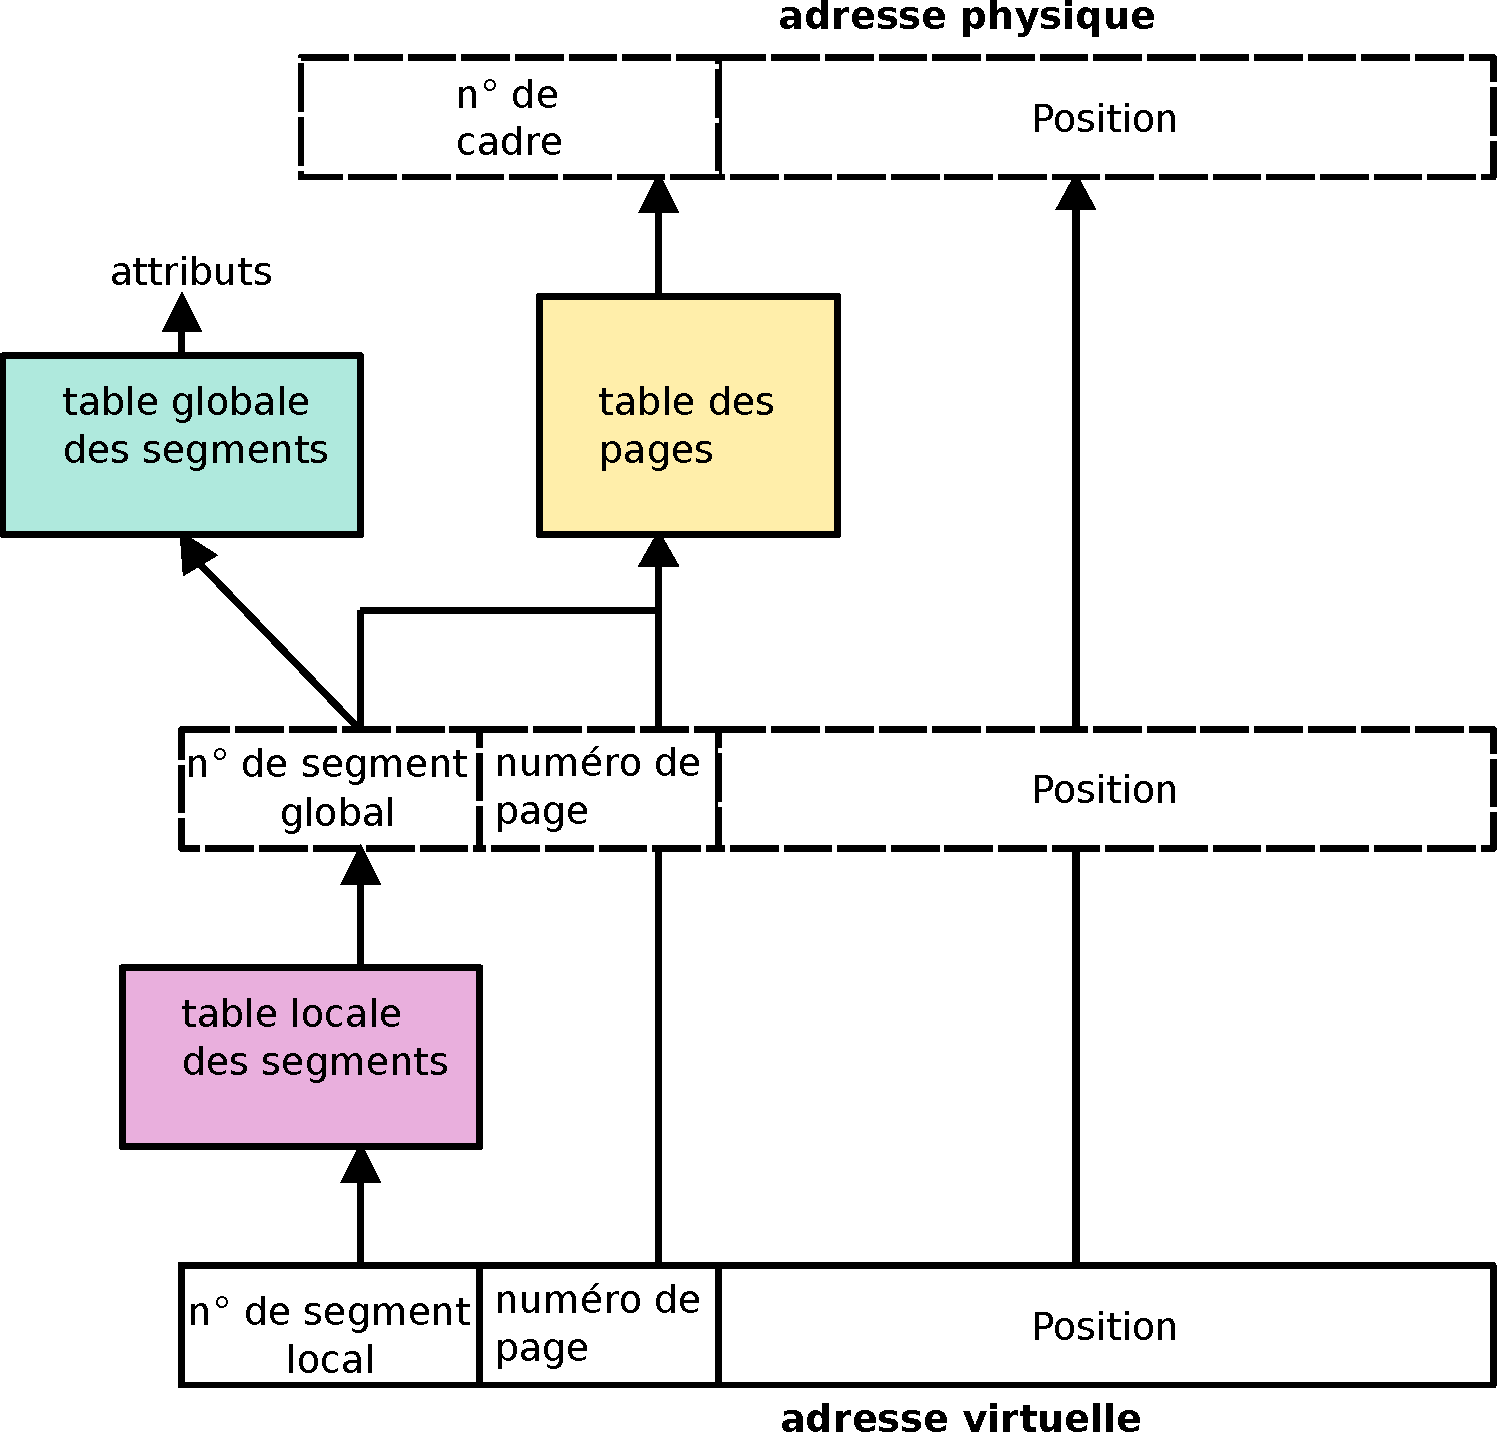
\includegraphics[width=0.7\linewidth]{fig2/generation-mv}
  \end{figure}
\end{frame}

\begin{frame}
  \frametitle{Combinaison avec le swapping}
  \begin{figure}
    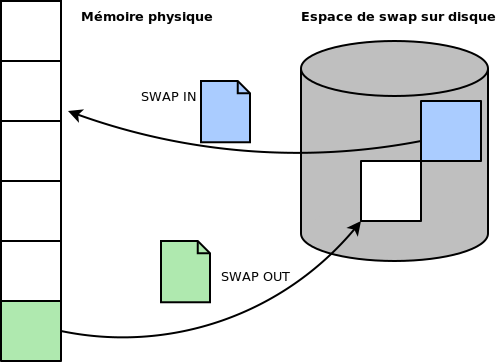
\includegraphics[width=0.8\linewidth]{fig2/swapping}
  \end{figure}
\end{frame}

\begin{frame}
  \frametitle{Bilan}
  Combinaison de~:
  \begin{itemize}
  \item pagination, 
  \item segmentation, 
  \item swapping
  \end{itemize}
  \vspace{0.5cm}
  
  Permet~:
  \begin{itemize}
  \item la cohabitation entre les processus
  \item la protection
  \item les zones partagées
  \item l'économie mémoire
  \end{itemize}
  \vspace{0.5cm}
  
  Technique largement adoptée depuis les années 70
\end{frame}
\end{document}

% LocalWords:  oeuf-colomb.jpg pagination.png format-pagination.png MMU memory
% LocalWords:  generation-pagination.png swapping mapping swapping.png blue ASR
% LocalWords:  segmentée-paginée width memoire-images beamer hideallsubsections
% LocalWords:  currentsection hideothersubsections Michel Billaud Random Access
% LocalWords:  monotâches monotâche d'E multitâches multitâche Pb additionneur
% LocalWords:  dia-partage-memoire indep-code-adr-physique conv-log-phys frag
% LocalWords:  indep-code-adr-logique relocation first-fit best-fit worst-fit
% LocalWords:  buddy system quick-fit new delete swapping-segment seg num STBR
% LocalWords:  Segment-table register ségments length STLR Wikipedia TLS TGS
% LocalWords:  format-pagination generation-pagination FIFO LRU Last Recently
% LocalWords:  Used lontemps concervée NRU Not generation-mv
